\documentclass[]{article}
\usepackage{lmodern}
\usepackage{amssymb,amsmath}
\usepackage{ifxetex,ifluatex}
\usepackage{fixltx2e} % provides \textsubscript
\ifnum 0\ifxetex 1\fi\ifluatex 1\fi=0 % if pdftex
  \usepackage[T1]{fontenc}
  \usepackage[utf8]{inputenc}
\else % if luatex or xelatex
  \ifxetex
    \usepackage{mathspec}
  \else
    \usepackage{fontspec}
  \fi
  \defaultfontfeatures{Ligatures=TeX,Scale=MatchLowercase}
\fi
% use upquote if available, for straight quotes in verbatim environments
\IfFileExists{upquote.sty}{\usepackage{upquote}}{}
% use microtype if available
\IfFileExists{microtype.sty}{%
\usepackage{microtype}
\UseMicrotypeSet[protrusion]{basicmath} % disable protrusion for tt fonts
}{}
\usepackage[margin=1in]{geometry}
\usepackage{hyperref}
\hypersetup{unicode=true,
            pdftitle={Homework 4},
            pdfauthor={Yu-Jen Lin},
            pdfborder={0 0 0},
            breaklinks=true}
\urlstyle{same}  % don't use monospace font for urls
\usepackage{color}
\usepackage{fancyvrb}
\newcommand{\VerbBar}{|}
\newcommand{\VERB}{\Verb[commandchars=\\\{\}]}
\DefineVerbatimEnvironment{Highlighting}{Verbatim}{commandchars=\\\{\}}
% Add ',fontsize=\small' for more characters per line
\usepackage{framed}
\definecolor{shadecolor}{RGB}{248,248,248}
\newenvironment{Shaded}{\begin{snugshade}}{\end{snugshade}}
\newcommand{\KeywordTok}[1]{\textcolor[rgb]{0.13,0.29,0.53}{\textbf{{#1}}}}
\newcommand{\DataTypeTok}[1]{\textcolor[rgb]{0.13,0.29,0.53}{{#1}}}
\newcommand{\DecValTok}[1]{\textcolor[rgb]{0.00,0.00,0.81}{{#1}}}
\newcommand{\BaseNTok}[1]{\textcolor[rgb]{0.00,0.00,0.81}{{#1}}}
\newcommand{\FloatTok}[1]{\textcolor[rgb]{0.00,0.00,0.81}{{#1}}}
\newcommand{\ConstantTok}[1]{\textcolor[rgb]{0.00,0.00,0.00}{{#1}}}
\newcommand{\CharTok}[1]{\textcolor[rgb]{0.31,0.60,0.02}{{#1}}}
\newcommand{\SpecialCharTok}[1]{\textcolor[rgb]{0.00,0.00,0.00}{{#1}}}
\newcommand{\StringTok}[1]{\textcolor[rgb]{0.31,0.60,0.02}{{#1}}}
\newcommand{\VerbatimStringTok}[1]{\textcolor[rgb]{0.31,0.60,0.02}{{#1}}}
\newcommand{\SpecialStringTok}[1]{\textcolor[rgb]{0.31,0.60,0.02}{{#1}}}
\newcommand{\ImportTok}[1]{{#1}}
\newcommand{\CommentTok}[1]{\textcolor[rgb]{0.56,0.35,0.01}{\textit{{#1}}}}
\newcommand{\DocumentationTok}[1]{\textcolor[rgb]{0.56,0.35,0.01}{\textbf{\textit{{#1}}}}}
\newcommand{\AnnotationTok}[1]{\textcolor[rgb]{0.56,0.35,0.01}{\textbf{\textit{{#1}}}}}
\newcommand{\CommentVarTok}[1]{\textcolor[rgb]{0.56,0.35,0.01}{\textbf{\textit{{#1}}}}}
\newcommand{\OtherTok}[1]{\textcolor[rgb]{0.56,0.35,0.01}{{#1}}}
\newcommand{\FunctionTok}[1]{\textcolor[rgb]{0.00,0.00,0.00}{{#1}}}
\newcommand{\VariableTok}[1]{\textcolor[rgb]{0.00,0.00,0.00}{{#1}}}
\newcommand{\ControlFlowTok}[1]{\textcolor[rgb]{0.13,0.29,0.53}{\textbf{{#1}}}}
\newcommand{\OperatorTok}[1]{\textcolor[rgb]{0.81,0.36,0.00}{\textbf{{#1}}}}
\newcommand{\BuiltInTok}[1]{{#1}}
\newcommand{\ExtensionTok}[1]{{#1}}
\newcommand{\PreprocessorTok}[1]{\textcolor[rgb]{0.56,0.35,0.01}{\textit{{#1}}}}
\newcommand{\AttributeTok}[1]{\textcolor[rgb]{0.77,0.63,0.00}{{#1}}}
\newcommand{\RegionMarkerTok}[1]{{#1}}
\newcommand{\InformationTok}[1]{\textcolor[rgb]{0.56,0.35,0.01}{\textbf{\textit{{#1}}}}}
\newcommand{\WarningTok}[1]{\textcolor[rgb]{0.56,0.35,0.01}{\textbf{\textit{{#1}}}}}
\newcommand{\AlertTok}[1]{\textcolor[rgb]{0.94,0.16,0.16}{{#1}}}
\newcommand{\ErrorTok}[1]{\textcolor[rgb]{0.64,0.00,0.00}{\textbf{{#1}}}}
\newcommand{\NormalTok}[1]{{#1}}
\usepackage{graphicx,grffile}
\makeatletter
\def\maxwidth{\ifdim\Gin@nat@width>\linewidth\linewidth\else\Gin@nat@width\fi}
\def\maxheight{\ifdim\Gin@nat@height>\textheight\textheight\else\Gin@nat@height\fi}
\makeatother
% Scale images if necessary, so that they will not overflow the page
% margins by default, and it is still possible to overwrite the defaults
% using explicit options in \includegraphics[width, height, ...]{}
\setkeys{Gin}{width=\maxwidth,height=\maxheight,keepaspectratio}
\IfFileExists{parskip.sty}{%
\usepackage{parskip}
}{% else
\setlength{\parindent}{0pt}
\setlength{\parskip}{6pt plus 2pt minus 1pt}
}
\setlength{\emergencystretch}{3em}  % prevent overfull lines
\providecommand{\tightlist}{%
  \setlength{\itemsep}{0pt}\setlength{\parskip}{0pt}}
\setcounter{secnumdepth}{0}
% Redefines (sub)paragraphs to behave more like sections
\ifx\paragraph\undefined\else
\let\oldparagraph\paragraph
\renewcommand{\paragraph}[1]{\oldparagraph{#1}\mbox{}}
\fi
\ifx\subparagraph\undefined\else
\let\oldsubparagraph\subparagraph
\renewcommand{\subparagraph}[1]{\oldsubparagraph{#1}\mbox{}}
\fi

%%% Use protect on footnotes to avoid problems with footnotes in titles
\let\rmarkdownfootnote\footnote%
\def\footnote{\protect\rmarkdownfootnote}

%%% Change title format to be more compact
\usepackage{titling}

% Create subtitle command for use in maketitle
\newcommand{\subtitle}[1]{
  \posttitle{
    \begin{center}\large#1\end{center}
    }
}

\setlength{\droptitle}{-2em}
  \title{Homework 4}
  \pretitle{\vspace{\droptitle}\centering\huge}
  \posttitle{\par}
  \author{Yu-Jen Lin}
  \preauthor{\centering\large\emph}
  \postauthor{\par}
  \date{}
  \predate{}\postdate{}


\begin{document}
\maketitle

\paragraph{\texorpdfstring{\href{mailto:b04b01036@ntu.edu.tw}{\nolinkurl{b04b01036@ntu.edu.tw}}}{b04b01036@ntu.edu.tw}}\label{b04b01036ntu.edu.tw}

\paragraph{--------------------------------------------------------------------------------------------------------------------------------------------------------}\label{section}

\paragraph{Set working directory}\label{set-working-directory}

\begin{Shaded}
\begin{Highlighting}[]
\KeywordTok{setwd}\NormalTok{(}\StringTok{"~/R"}\NormalTok{)}
\end{Highlighting}
\end{Shaded}

\paragraph{Read enviANDdensity.csv into
R}\label{read-envianddensity.csv-into-r}

\begin{Shaded}
\begin{Highlighting}[]
\NormalTok{enviANDdensity <-}\StringTok{ }\KeywordTok{read.csv}\NormalTok{(}\DataTypeTok{file=}\StringTok{"~/R/enviANDdensity.csv"}\NormalTok{, }\DataTypeTok{header=}\OtherTok{TRUE}\NormalTok{)}
\end{Highlighting}
\end{Shaded}

Because we only need the data in ``FishDensity..ind..1000m3.'' and
``CopepodDensity.ind..m3.'', I take these two columns out and set as
``FishDensity'' and ``CopepodDensity'' separately.

\begin{Shaded}
\begin{Highlighting}[]
\NormalTok{FishDensity <-}\StringTok{ }\NormalTok{enviANDdensity$FishDensity..ind..1000m3.}
\NormalTok{CopepodDensity <-}\StringTok{ }\NormalTok{enviANDdensity$CopepodDensity.ind..m3.}
\end{Highlighting}
\end{Shaded}

\paragraph{Re-do HW3 {[}Normal theory{]} mean and
SE(mean)}\label{re-do-hw3-normal-theory-mean-and-semean}

\begin{Shaded}
\begin{Highlighting}[]
\NormalTok{FishDensity.mean <-}\StringTok{ }\KeywordTok{mean}\NormalTok{(FishDensity)}
\NormalTok{FishDensity.mean}
\end{Highlighting}
\end{Shaded}

\begin{verbatim}
## [1] 322.4516
\end{verbatim}

\begin{Shaded}
\begin{Highlighting}[]
\NormalTok{FishDensity.SE <-}\StringTok{ }\KeywordTok{var}\NormalTok{(FishDensity)^}\FloatTok{0.5}\NormalTok{/}\KeywordTok{length}\NormalTok{(FishDensity)^}\FloatTok{0.5}
\NormalTok{FishDensity.SE}
\end{Highlighting}
\end{Shaded}

\begin{verbatim}
## [1] 61.23107
\end{verbatim}

\begin{Shaded}
\begin{Highlighting}[]
\NormalTok{CopepodDensity.mean <-}\StringTok{ }\KeywordTok{mean}\NormalTok{(CopepodDensity)}
\NormalTok{CopepodDensity.mean}
\end{Highlighting}
\end{Shaded}

\begin{verbatim}
## [1] 1972.374
\end{verbatim}

\begin{Shaded}
\begin{Highlighting}[]
\NormalTok{CopepodDensity.SE <-}\StringTok{ }\KeywordTok{var}\NormalTok{(CopepodDensity)^}\FloatTok{0.5}\NormalTok{/}\KeywordTok{length}\NormalTok{(CopepodDensity)^}\FloatTok{0.5}
\NormalTok{CopepodDensity.SE}
\end{Highlighting}
\end{Shaded}

\begin{verbatim}
## [1] 342.5549
\end{verbatim}

-------------------------------------------------------------------------------------------------------------------------------------------------------------------------------------------------------------------------------------

\paragraph{1. Compute the mean and stand error of the mean for the fish
and copepod density (all data points) respectively using Jackknife. Plot
the histogram of Jackknife
means.}\label{compute-the-mean-and-stand-error-of-the-mean-for-the-fish-and-copepod-density-all-data-points-respectively-using-jackknife.-plot-the-histogram-of-jackknife-means.}

\paragraph{{[}Jackknife{]} mean and stand error of the
mean}\label{jackknife-mean-and-stand-error-of-the-mean}

\begin{enumerate}
\def\labelenumi{(\arabic{enumi})}
\tightlist
\item
  FishDensity
\end{enumerate}

\begin{Shaded}
\begin{Highlighting}[]
\NormalTok{FishDensity.Jackknife.means <-}\StringTok{ }\KeywordTok{c}\NormalTok{() }\CommentTok{# set a vector to put the following sampling results}

\NormalTok{for (i in }\DecValTok{1}\NormalTok{:}\KeywordTok{length}\NormalTok{(FishDensity)) \{}
\NormalTok{FishDensity.Jackknife.i <-}\StringTok{ }\NormalTok{FishDensity[-i] }\CommentTok{# single sampling result}
\NormalTok{FishDensity.Jackknife.means[i] <-}\StringTok{ }\KeywordTok{mean}\NormalTok{(FishDensity.Jackknife.i) }\CommentTok{# put every mean of every single result into the vector I've created}
\NormalTok{\}}

\NormalTok{FishDensity.Jackknife.means.mean <-}\StringTok{ }\KeywordTok{mean}\NormalTok{(FishDensity.Jackknife.means) }\CommentTok{# mean of Jackknife means}
\NormalTok{FishDensity.Jackknife.means.mean}
\end{Highlighting}
\end{Shaded}

\begin{verbatim}
## [1] 322.4516
\end{verbatim}

\begin{Shaded}
\begin{Highlighting}[]
\NormalTok{FishDensity.Jackknife.means.SE <-}\StringTok{ }\KeywordTok{var}\NormalTok{(FishDensity.Jackknife.means)^}\FloatTok{0.5}

\CommentTok{# calculate SE}
\NormalTok{sum.F =}\StringTok{ }\DecValTok{0}
\NormalTok{for (i in }\DecValTok{1}\NormalTok{:}\KeywordTok{length}\NormalTok{(FishDensity)) \{}
  \NormalTok{sum.F.i <-}\StringTok{ }\NormalTok{(FishDensity.Jackknife.means[i] -}\StringTok{ }\NormalTok{FishDensity.Jackknife.means.mean)^}\DecValTok{2}
  \NormalTok{sum.F <-}\StringTok{ }\NormalTok{sum.F +}\StringTok{ }\NormalTok{sum.F.i}
\NormalTok{\}}
\NormalTok{FishDensity.Jackknife.means.SE <-(sum.F*(}\DecValTok{34-1}\NormalTok{)/}\DecValTok{34}\NormalTok{) ^}\StringTok{ }\FloatTok{0.5}
\NormalTok{FishDensity.Jackknife.means.SE}
\end{Highlighting}
\end{Shaded}

\begin{verbatim}
## [1] 61.23107
\end{verbatim}

\begin{enumerate}
\def\labelenumi{(\arabic{enumi})}
\setcounter{enumi}{1}
\tightlist
\item
  CopepodDensity
\end{enumerate}

\begin{Shaded}
\begin{Highlighting}[]
\NormalTok{CopepodDensity.Jackknife.means <-}\StringTok{ }\KeywordTok{c}\NormalTok{() }\CommentTok{# set a vector to put the following sampling results}

\NormalTok{for (i in }\DecValTok{1}\NormalTok{:}\KeywordTok{length}\NormalTok{(CopepodDensity)) \{}
\NormalTok{CopepodDensity.Jackknife.i <-}\StringTok{ }\NormalTok{CopepodDensity[-i] }\CommentTok{# single sampling result}
\NormalTok{CopepodDensity.Jackknife.means[i] <-}\StringTok{ }\KeywordTok{mean}\NormalTok{(CopepodDensity.Jackknife.i) }\CommentTok{# put every mean of every single result into the vector I've created}
\NormalTok{\}}

\NormalTok{CopepodDensity.Jackknife.means.mean <-}\StringTok{ }\KeywordTok{mean}\NormalTok{(CopepodDensity.Jackknife.means) }\CommentTok{# mean of Jackknife means}
\NormalTok{CopepodDensity.Jackknife.means.mean}
\end{Highlighting}
\end{Shaded}

\begin{verbatim}
## [1] 1972.374
\end{verbatim}

\begin{Shaded}
\begin{Highlighting}[]
\CommentTok{# calculate SE}
\NormalTok{sum.C =}\StringTok{ }\DecValTok{0}
\NormalTok{for (i in }\DecValTok{1}\NormalTok{:}\KeywordTok{length}\NormalTok{(CopepodDensity)) \{}
  \NormalTok{sum.C.i <-}\StringTok{ }\NormalTok{(CopepodDensity.Jackknife.means[i] -}\StringTok{ }\NormalTok{CopepodDensity.Jackknife.means.mean)^}\DecValTok{2}
  \NormalTok{sum.C <-}\StringTok{ }\NormalTok{sum.C +}\StringTok{ }\NormalTok{sum.C.i}
\NormalTok{\}}
\NormalTok{CopepodDensity.Jackknife.means.SE <-(sum.C*(}\DecValTok{34-1}\NormalTok{)/}\DecValTok{34}\NormalTok{) ^}\StringTok{ }\FloatTok{0.5}
\NormalTok{CopepodDensity.Jackknife.means.SE}
\end{Highlighting}
\end{Shaded}

\begin{verbatim}
## [1] 342.5549
\end{verbatim}

\paragraph{plot the histogram}\label{plot-the-histogram}

I plot the histogram of Jackknife. The blue line is the mean of
Jackknife means. The black line is the mean calculated by normal theory.
We can see that they are really close to each other. When we compare
histogram of jackknife with bootstrap, we find jackknife results are
less likely to form a normal distribution than bootstrap because the
sample size of jackknife is far smaller than bootstrap.

\begin{enumerate}
\def\labelenumi{(\arabic{enumi})}
\tightlist
\item
  FishDensity means by \href{blue}{Jackknife} or \href{black}{Normal
  Theory}
\end{enumerate}

\begin{Shaded}
\begin{Highlighting}[]
\KeywordTok{hist}\NormalTok{(FishDensity.Jackknife.means)}
\KeywordTok{abline}\NormalTok{(}\DataTypeTok{v =} \NormalTok{FishDensity.mean, }\DataTypeTok{col =} \StringTok{"black"}\NormalTok{, }\DataTypeTok{lwd =} \DecValTok{2}\NormalTok{)}
\KeywordTok{abline}\NormalTok{(}\DataTypeTok{v =} \NormalTok{FishDensity.Jackknife.means.mean, }\DataTypeTok{col =} \StringTok{"blue"}\NormalTok{, }\DataTypeTok{lwd =} \DecValTok{2}\NormalTok{)}
\end{Highlighting}
\end{Shaded}

\includegraphics{20180322_HW4-2_files/figure-latex/unnamed-chunk-7-1.pdf}

\begin{enumerate}
\def\labelenumi{(\arabic{enumi})}
\setcounter{enumi}{1}
\tightlist
\item
  CopepodDensity means by \href{blue}{Jackknife} or \href{black}{Normal
  Theory}
\end{enumerate}

\begin{Shaded}
\begin{Highlighting}[]
\KeywordTok{hist}\NormalTok{(CopepodDensity.Jackknife.means)}
\KeywordTok{abline}\NormalTok{(}\DataTypeTok{v =} \NormalTok{CopepodDensity.mean, }\DataTypeTok{col =} \StringTok{"black"}\NormalTok{, }\DataTypeTok{lwd =} \DecValTok{2}\NormalTok{)}
\KeywordTok{abline}\NormalTok{(}\DataTypeTok{v =} \NormalTok{CopepodDensity.Jackknife.means.mean, }\DataTypeTok{col =} \StringTok{"blue"}\NormalTok{, }\DataTypeTok{lwd =} \DecValTok{2}\NormalTok{)}
\end{Highlighting}
\end{Shaded}

\includegraphics{20180322_HW4-2_files/figure-latex/unnamed-chunk-8-1.pdf}

-------------------------------------------------------------------------------------------------------------------------------------------------------------------------------------------------------------------------------------

\paragraph{2. Compute the regression coefficients
for}\label{compute-the-regression-coefficients-for}

\paragraph{fish = β0+β1*copepod and Jackknife SE of β0 and β1. \#\#\#\#
Plot the histogram of Jackknife β0 and
β1.}\label{fish-01copepod-and-jackknife-se-of-0-and-1.-plot-the-histogram-of-jackknife-0-and-1.}

\paragraph{Compute the regression coefficients
for}\label{compute-the-regression-coefficients-for-1}

\paragraph{fish(y) = β0 + β1 * copepod(x).}\label{fishy-0-1-copepodx.}

Dimension of y -\textgreater{} (n,1) Dimension of β0 -\textgreater{}
(n,1) Dimension of β1 -\textgreater{} (k+1,1) Dimension of X
-\textgreater{} (n,k+1)

\begin{Shaded}
\begin{Highlighting}[]
\NormalTok{n <-}\StringTok{ }\KeywordTok{length}\NormalTok{(FishDensity)}
\NormalTok{k <-}\StringTok{ }\DecValTok{1}

\NormalTok{y  <-}\StringTok{ }\KeywordTok{matrix}\NormalTok{(FishDensity, }\DataTypeTok{nrow=}\NormalTok{n, }\DataTypeTok{ncol=}\DecValTok{1}\NormalTok{, }\DataTypeTok{byrow =} \OtherTok{TRUE}\NormalTok{) }\CommentTok{# put the original sample into y}
\NormalTok{x  <-}\StringTok{ }\KeywordTok{matrix}\NormalTok{(}\KeywordTok{c}\NormalTok{(}\KeywordTok{rep}\NormalTok{(}\DecValTok{1}\NormalTok{, }\DataTypeTok{times=}\NormalTok{n),CopepodDensity), }\DataTypeTok{nrow=}\NormalTok{n, }\DataTypeTok{ncol=}\NormalTok{k}\DecValTok{+1}\NormalTok{, }\DataTypeTok{byrow =} \OtherTok{FALSE}\NormalTok{)  }\CommentTok{# put the original sample into x}

\NormalTok{β}\DecValTok{1} \NormalTok{<-}\StringTok{ }\KeywordTok{solve}\NormalTok{(}\KeywordTok{t}\NormalTok{(x) %*%}\StringTok{ }\NormalTok{x) %*%}\StringTok{ }\KeywordTok{t}\NormalTok{(x) %*%}\StringTok{ }\NormalTok{y}
\NormalTok{β}\DecValTok{1}
\end{Highlighting}
\end{Shaded}

\begin{verbatim}
##            [,1]
## [1,] 93.0646559
## [2,]  0.1162999
\end{verbatim}

\begin{Shaded}
\begin{Highlighting}[]
\NormalTok{β}\DecValTok{0} \NormalTok{<-}\StringTok{ }\NormalTok{y -}\StringTok{ }\NormalTok{x %*%}\StringTok{ }\NormalTok{β}\DecValTok{1}  \CommentTok{# fish(y) = β0 + β1 * copepod(x)}
\end{Highlighting}
\end{Shaded}

Thus, through β1, I found the intercept of the regression line is
93.0647 and the slope of the regression line is 0.1163. y = 93.0647 +
0.1163*x

\paragraph{Plot fish (dependent) v.s. copepod (independent) and the
regression
line.}\label{plot-fish-dependent-v.s.-copepod-independent-and-the-regression-line.}

I plot the regression line I just computed in below. (blue) y = 93.0647
+ 0.1163*x

\begin{Shaded}
\begin{Highlighting}[]
\KeywordTok{plot}\NormalTok{(CopepodDensity, FishDensity, }\DataTypeTok{main=}\StringTok{"Fish v.s. Copepod"}\NormalTok{, }
    \DataTypeTok{xlab=}\StringTok{"Copepod Density (/m3) "}\NormalTok{, }\DataTypeTok{ylab=}\StringTok{"Fish Density (/1000m3) "}\NormalTok{, }\DataTypeTok{pch=}\DecValTok{19}\NormalTok{)}
\KeywordTok{abline}\NormalTok{(}\DataTypeTok{a=}\FloatTok{93.0647}\NormalTok{, }\DataTypeTok{b=}\FloatTok{0.1163}\NormalTok{, }\DataTypeTok{col=}\StringTok{"blue"}\NormalTok{) }\CommentTok{# regression line (y~x) # the regression line I computed in previous step, a=intercept b=slope}
\end{Highlighting}
\end{Shaded}

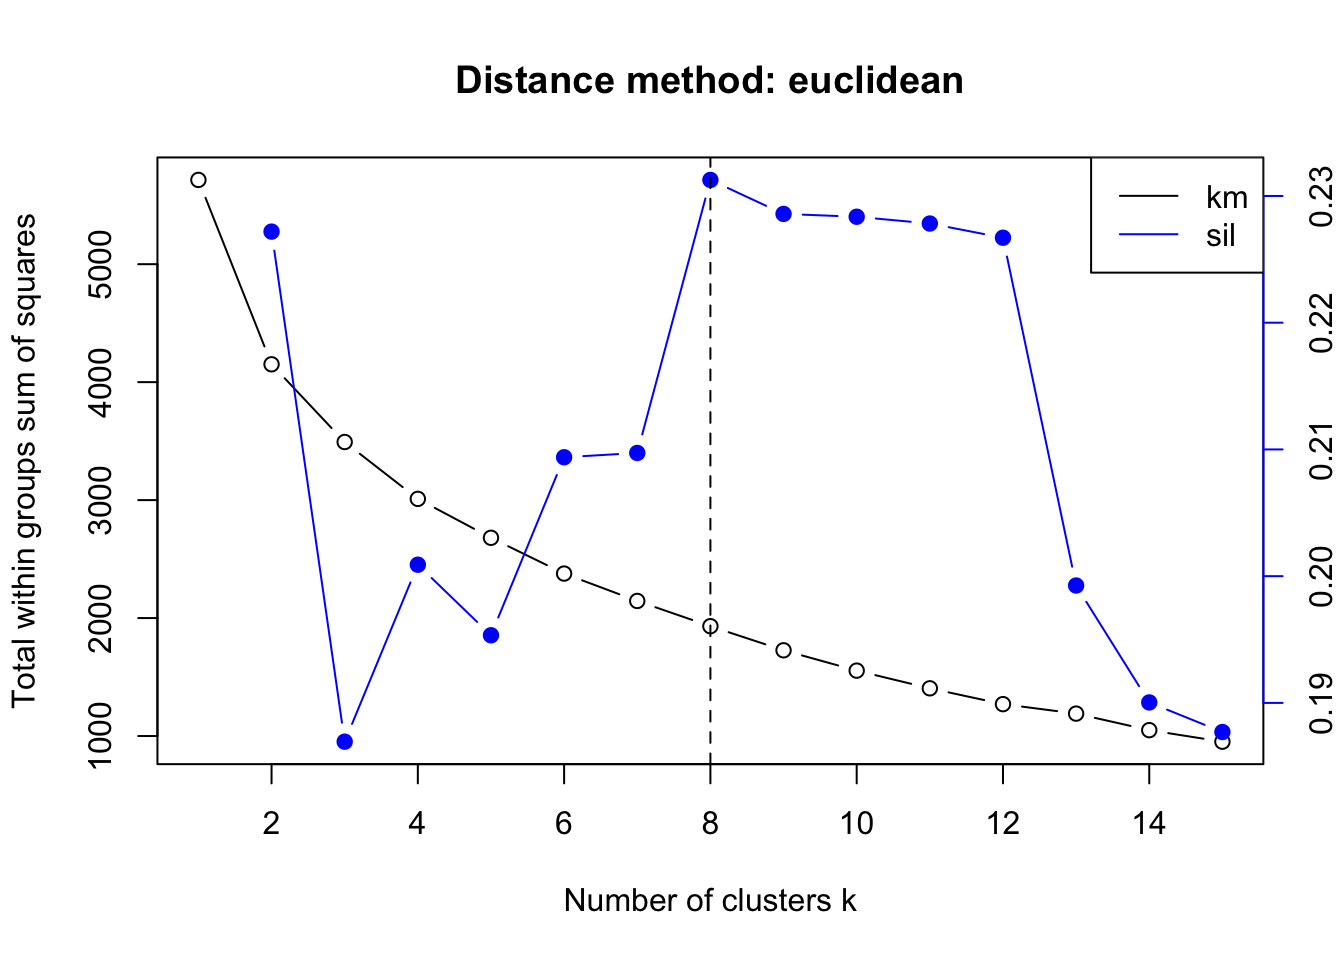
\includegraphics{20180322_HW4-2_files/figure-latex/unnamed-chunk-10-1.pdf}

\paragraph{{[}Jackknife{]} SE(β0) and
SE(β1).}\label{jackknife-se0-and-se1.}

\begin{Shaded}
\begin{Highlighting}[]
\CommentTok{# set vectors to put the following sampling results}
\NormalTok{Jackknife.β}\DecValTok{0} \NormalTok{<-}\StringTok{ }\KeywordTok{c}\NormalTok{() }
\NormalTok{Jackknife.β}\DecValTok{1} \NormalTok{<-}\StringTok{ }\KeywordTok{c}\NormalTok{()}

\CommentTok{# set starting points}
\NormalTok{n.jn <-}\StringTok{ }\KeywordTok{length}\NormalTok{(FishDensity)-}\DecValTok{1}
\NormalTok{k.jn <-}\StringTok{ }\KeywordTok{length}\NormalTok{(FishDensity) }

\CommentTok{# Jackknife}
\NormalTok{for (i in }\DecValTok{1}\NormalTok{:k.jn) \{}
\NormalTok{Jackknife.Fish.i <-}\StringTok{ }\NormalTok{FishDensity[-i] }\CommentTok{# single sampling result}
\NormalTok{Jackknife.Copepod.i <-}\StringTok{ }\NormalTok{CopepodDensity[-i] }\CommentTok{# single sampling result}

\NormalTok{y.jn  <-}\StringTok{ }\KeywordTok{matrix}\NormalTok{(Jackknife.Fish.i, }\DataTypeTok{nrow=}\NormalTok{n.jn, }\DataTypeTok{ncol=}\DecValTok{1}\NormalTok{, }\DataTypeTok{byrow =} \OtherTok{FALSE}\NormalTok{) }\CommentTok{# put the Jackknife sample into y.jn}
\NormalTok{x.jn  <-}\StringTok{ }\KeywordTok{cbind}\NormalTok{(}\KeywordTok{c}\NormalTok{(}\KeywordTok{rep}\NormalTok{(}\DecValTok{1}\NormalTok{, }\DataTypeTok{times=}\NormalTok{n.jn)), }\KeywordTok{as.matrix}\NormalTok{(Jackknife.Copepod.i)) }\CommentTok{# combine the new column into the x.jn}

\NormalTok{β}\FloatTok{1.}\NormalTok{jn <-}\StringTok{ }\KeywordTok{solve}\NormalTok{(}\KeywordTok{t}\NormalTok{(x.jn) %*%}\StringTok{ }\NormalTok{x.jn) %*%}\StringTok{ }\KeywordTok{t}\NormalTok{(x.jn) %*%}\StringTok{ }\NormalTok{y.jn}
\NormalTok{Jackknife.β}\DecValTok{0}\NormalTok{[i] <-}\StringTok{ }\NormalTok{β}\FloatTok{1.}\NormalTok{jn[}\DecValTok{1}\NormalTok{] }\CommentTok{# intercept}
\NormalTok{Jackknife.β}\DecValTok{1}\NormalTok{[i] <-}\StringTok{ }\NormalTok{β}\FloatTok{1.}\NormalTok{jn[}\DecValTok{2}\NormalTok{] }\CommentTok{# slope}
\NormalTok{\}}

\NormalTok{Jackknife.β}\FloatTok{0.}\NormalTok{mean <-}\StringTok{ }\KeywordTok{mean}\NormalTok{(Jackknife.β}\DecValTok{0}\NormalTok{)}
\NormalTok{Jackknife.β}\FloatTok{0.}\NormalTok{mean}
\end{Highlighting}
\end{Shaded}

\begin{verbatim}
## [1] 92.73093
\end{verbatim}

\begin{Shaded}
\begin{Highlighting}[]
\NormalTok{Jackknife.β}\FloatTok{1.}\NormalTok{mean <-}\StringTok{ }\KeywordTok{mean}\NormalTok{(Jackknife.β}\DecValTok{1}\NormalTok{)}
\NormalTok{Jackknife.β}\FloatTok{1.}\NormalTok{mean}
\end{Highlighting}
\end{Shaded}

\begin{verbatim}
## [1] 0.1165492
\end{verbatim}

\begin{Shaded}
\begin{Highlighting}[]
\CommentTok{# calculate SE}
\NormalTok{sum.β}\FloatTok{0.}\NormalTok{J =}\StringTok{ }\DecValTok{0}
\NormalTok{for (i in }\DecValTok{1}\NormalTok{:}\KeywordTok{length}\NormalTok{(Jackknife.β}\DecValTok{0}\NormalTok{)) \{}
  \NormalTok{sum.β}\FloatTok{0.}\NormalTok{J.i <-}\StringTok{ }\NormalTok{(Jackknife.β}\DecValTok{0}\NormalTok{[i] -}\StringTok{ }\KeywordTok{mean}\NormalTok{(Jackknife.β}\DecValTok{0}\NormalTok{))^}\DecValTok{2}
  \NormalTok{sum.β}\FloatTok{0.}\NormalTok{J <-}\StringTok{ }\NormalTok{sum.β}\FloatTok{0.}\NormalTok{J +}\StringTok{ }\NormalTok{sum.β}\FloatTok{0.}\NormalTok{J.i}
\NormalTok{\}}
\NormalTok{Jackknife.β}\FloatTok{0.}\NormalTok{SE <-(sum.β}\FloatTok{0.}\NormalTok{J*(}\DecValTok{34-1}\NormalTok{)/}\DecValTok{34}\NormalTok{) ^}\StringTok{ }\FloatTok{0.5}
\NormalTok{Jackknife.β}\FloatTok{0.}\NormalTok{SE}
\end{Highlighting}
\end{Shaded}

\begin{verbatim}
## [1] 69.27329
\end{verbatim}

\begin{Shaded}
\begin{Highlighting}[]
\NormalTok{sum.β}\FloatTok{1.}\NormalTok{J =}\StringTok{ }\DecValTok{0}
\NormalTok{for (i in }\DecValTok{1}\NormalTok{:}\KeywordTok{length}\NormalTok{(Jackknife.β}\DecValTok{1}\NormalTok{)) \{}
  \NormalTok{sum.β}\FloatTok{1.}\NormalTok{J.i <-}\StringTok{ }\NormalTok{(Jackknife.β}\DecValTok{1}\NormalTok{[i] -}\StringTok{ }\KeywordTok{mean}\NormalTok{(Jackknife.β}\DecValTok{1}\NormalTok{))^}\DecValTok{2}
  \NormalTok{sum.β}\FloatTok{1.}\NormalTok{J <-}\StringTok{ }\NormalTok{sum.β}\FloatTok{1.}\NormalTok{J +}\StringTok{ }\NormalTok{sum.β}\FloatTok{1.}\NormalTok{J.i}
\NormalTok{\}}
\NormalTok{Jackknife.β}\FloatTok{1.}\NormalTok{SE <-(sum.β}\FloatTok{1.}\NormalTok{J*(}\DecValTok{34-1}\NormalTok{)/}\DecValTok{34}\NormalTok{) ^}\StringTok{ }\FloatTok{0.5}
\NormalTok{Jackknife.β}\FloatTok{1.}\NormalTok{SE}
\end{Highlighting}
\end{Shaded}

\begin{verbatim}
## [1] 0.0380003
\end{verbatim}

\paragraph{Plot the histogram of Jackknife β0 and
β1.}\label{plot-the-histogram-of-jackknife-0-and-1.}

Jackknife β0 means by \href{blue}{Jackknife} and \href{black}{Normal
Theory}

\begin{Shaded}
\begin{Highlighting}[]
\KeywordTok{hist}\NormalTok{(Jackknife.β}\DecValTok{0}\NormalTok{)}
\end{Highlighting}
\end{Shaded}

\begin{verbatim}
## Warning in title(main = main, sub = sub, xlab = xlab, ylab = ylab, ...):
## conversion failure on 'Histogram of Jackknife.β0' in 'mbcsToSbcs': dot
## substituted for <ce>
\end{verbatim}

\begin{verbatim}
## Warning in title(main = main, sub = sub, xlab = xlab, ylab = ylab, ...):
## conversion failure on 'Histogram of Jackknife.β0' in 'mbcsToSbcs': dot
## substituted for <b2>
\end{verbatim}

\begin{verbatim}
## Warning in title(main = main, sub = sub, xlab = xlab, ylab = ylab, ...):
## conversion failure on 'Jackknife.β0' in 'mbcsToSbcs': dot substituted for
## <ce>
\end{verbatim}

\begin{verbatim}
## Warning in title(main = main, sub = sub, xlab = xlab, ylab = ylab, ...):
## conversion failure on 'Jackknife.β0' in 'mbcsToSbcs': dot substituted for
## <b2>
\end{verbatim}

\begin{Shaded}
\begin{Highlighting}[]
\KeywordTok{abline}\NormalTok{(}\DataTypeTok{v =} \NormalTok{β}\DecValTok{1}\NormalTok{[}\DecValTok{1}\NormalTok{], }\DataTypeTok{col =} \StringTok{"black"}\NormalTok{, }\DataTypeTok{lwd =} \DecValTok{2}\NormalTok{) }\CommentTok{# mean calculated by Normal Theory}
\KeywordTok{abline}\NormalTok{(}\DataTypeTok{v =} \NormalTok{Jackknife.β}\FloatTok{0.}\NormalTok{mean, }\DataTypeTok{col =} \StringTok{"blue"}\NormalTok{, }\DataTypeTok{lwd =} \DecValTok{2}\NormalTok{) }\CommentTok{# mean calculated by Jackknife}
\end{Highlighting}
\end{Shaded}

\includegraphics{20180322_HW4-2_files/figure-latex/unnamed-chunk-12-1.pdf}

Jackknife β1 means by \href{blue}{Jackknife} and \href{black}{Normal
Theory}

\begin{Shaded}
\begin{Highlighting}[]
\KeywordTok{hist}\NormalTok{(Jackknife.β}\DecValTok{1}\NormalTok{)}
\end{Highlighting}
\end{Shaded}

\begin{verbatim}
## Warning in title(main = main, sub = sub, xlab = xlab, ylab = ylab, ...):
## conversion failure on 'Histogram of Jackknife.β1' in 'mbcsToSbcs': dot
## substituted for <ce>
\end{verbatim}

\begin{verbatim}
## Warning in title(main = main, sub = sub, xlab = xlab, ylab = ylab, ...):
## conversion failure on 'Histogram of Jackknife.β1' in 'mbcsToSbcs': dot
## substituted for <b2>
\end{verbatim}

\begin{verbatim}
## Warning in title(main = main, sub = sub, xlab = xlab, ylab = ylab, ...):
## conversion failure on 'Jackknife.β1' in 'mbcsToSbcs': dot substituted for
## <ce>
\end{verbatim}

\begin{verbatim}
## Warning in title(main = main, sub = sub, xlab = xlab, ylab = ylab, ...):
## conversion failure on 'Jackknife.β1' in 'mbcsToSbcs': dot substituted for
## <b2>
\end{verbatim}

\begin{Shaded}
\begin{Highlighting}[]
\KeywordTok{abline}\NormalTok{(}\DataTypeTok{v =} \NormalTok{β}\DecValTok{1}\NormalTok{[}\DecValTok{2}\NormalTok{], }\DataTypeTok{col =} \StringTok{"black"}\NormalTok{, }\DataTypeTok{lwd =} \DecValTok{2}\NormalTok{) }\CommentTok{# mean calculated by Normal Theory}
\KeywordTok{abline}\NormalTok{(}\DataTypeTok{v =} \NormalTok{Jackknife.β}\FloatTok{1.}\NormalTok{mean, }\DataTypeTok{col =} \StringTok{"blue"}\NormalTok{, }\DataTypeTok{lwd =} \DecValTok{2}\NormalTok{) }\CommentTok{# mean calculated by Jackknife}
\end{Highlighting}
\end{Shaded}

\includegraphics{20180322_HW4-2_files/figure-latex/unnamed-chunk-13-1.pdf}

-------------------------------------------------------------------------------------------------------------------------------------------------------------------------------------------------------------------------------------

\paragraph{Re-do HW3 {[}bootstrap{]} mean and
SE(mean)}\label{re-do-hw3-bootstrap-mean-and-semean}

\begin{enumerate}
\def\labelenumi{(\arabic{enumi})}
\tightlist
\item
  FishDensity bootstrap means
\end{enumerate}

\begin{Shaded}
\begin{Highlighting}[]
\NormalTok{FishDensity.bootstrap.means <-}\StringTok{ }\KeywordTok{c}\NormalTok{() }\CommentTok{# set a vector to put the following sampling results}
\NormalTok{for (i in }\DecValTok{1}\NormalTok{:}\DecValTok{999}\NormalTok{) \{}
\NormalTok{random <-}\StringTok{ }\KeywordTok{ceiling}\NormalTok{(}\KeywordTok{runif}\NormalTok{(}\DecValTok{34}\NormalTok{, }\DataTypeTok{min=}\DecValTok{0}\NormalTok{, }\DataTypeTok{max=}\DecValTok{34}\NormalTok{))}
\NormalTok{bootstrap.i <-}\StringTok{ }\NormalTok{FishDensity[random] }\CommentTok{# single sampling result}
\NormalTok{FishDensity.bootstrap.means[i] <-}\StringTok{ }\KeywordTok{mean}\NormalTok{(bootstrap.i) }\CommentTok{# put every mean of every single result into the vector I've created}
\NormalTok{\}}
\NormalTok{FishDensity.bootstrap.means <-}\StringTok{ }\KeywordTok{append}\NormalTok{(FishDensity.bootstrap.means, FishDensity.mean) }\CommentTok{# add the mean calculated by normal theory (total:1000)}
\NormalTok{FishDensity.bootstrap.means.mean <-}\StringTok{ }\KeywordTok{mean}\NormalTok{(FishDensity.bootstrap.means) }\CommentTok{# mean of bootstrap means}
\NormalTok{FishDensity.bootstrap.means.mean}
\end{Highlighting}
\end{Shaded}

\begin{verbatim}
## [1] 324.7612
\end{verbatim}

\begin{Shaded}
\begin{Highlighting}[]
\NormalTok{FishDensity.bootstrap.means.SE <-}\StringTok{ }\KeywordTok{var}\NormalTok{(FishDensity.bootstrap.means)^}\FloatTok{0.5}
\NormalTok{FishDensity.bootstrap.means.SE}
\end{Highlighting}
\end{Shaded}

\begin{verbatim}
## [1] 60.85436
\end{verbatim}

\begin{enumerate}
\def\labelenumi{(\arabic{enumi})}
\setcounter{enumi}{1}
\tightlist
\item
  CopepodDensity bootstrap means
\end{enumerate}

\begin{Shaded}
\begin{Highlighting}[]
\NormalTok{CopepodDensity.bootstrap.means <-}\StringTok{ }\KeywordTok{c}\NormalTok{() }\CommentTok{# set a vector to put the following sampling results}
\NormalTok{for (i in }\DecValTok{1}\NormalTok{:}\DecValTok{999}\NormalTok{) \{}
\NormalTok{random <-}\StringTok{ }\KeywordTok{ceiling}\NormalTok{(}\KeywordTok{runif}\NormalTok{(}\DecValTok{34}\NormalTok{, }\DataTypeTok{min=}\DecValTok{0}\NormalTok{, }\DataTypeTok{max=}\DecValTok{34}\NormalTok{))}
\NormalTok{bootstrap.i <-}\StringTok{ }\NormalTok{CopepodDensity[random] }\CommentTok{# single sampling result}
\NormalTok{CopepodDensity.bootstrap.means[i] <-}\StringTok{ }\KeywordTok{mean}\NormalTok{(bootstrap.i) }\CommentTok{# put every mean of every single result into the vector I've created}
\NormalTok{\}}
\NormalTok{CopepodDensity.bootstrap.means <-}\StringTok{ }\KeywordTok{append}\NormalTok{(CopepodDensity.bootstrap.means, CopepodDensity.mean) }\CommentTok{# add the mean calculated by normal theory (total:1000)}
\NormalTok{CopepodDensity.bootstrap.means.mean <-}\StringTok{ }\KeywordTok{mean}\NormalTok{(CopepodDensity.bootstrap.means) }\CommentTok{# mean of bootstrap means}
\NormalTok{CopepodDensity.bootstrap.means.mean}
\end{Highlighting}
\end{Shaded}

\begin{verbatim}
## [1] 1974.488
\end{verbatim}

\begin{Shaded}
\begin{Highlighting}[]
\NormalTok{CopepodDensity.bootstrap.means.SE <-}\StringTok{ }\KeywordTok{var}\NormalTok{(CopepodDensity.bootstrap.means)^}\FloatTok{0.5}
\NormalTok{CopepodDensity.bootstrap.means.SE}
\end{Highlighting}
\end{Shaded}

\begin{verbatim}
## [1] 332.6631
\end{verbatim}

-------------------------------------------------------------------------------------------------------------------------------------------------------------------------------------------------------------------------------------

\paragraph{Re-do HW3 {[}bootstrap{]} SE(β0) and
SE(β1).}\label{re-do-hw3-bootstrap-se0-and-se1.}

\begin{Shaded}
\begin{Highlighting}[]
\CommentTok{# set vectors to put the following sampling results}
\NormalTok{bootstrap.β}\DecValTok{0} \NormalTok{<-}\StringTok{ }\KeywordTok{c}\NormalTok{() }
\NormalTok{bootstrap.β}\DecValTok{1} \NormalTok{<-}\StringTok{ }\KeywordTok{c}\NormalTok{()}

\CommentTok{# set starting points}
\NormalTok{n.bt <-}\StringTok{ }\KeywordTok{length}\NormalTok{(FishDensity) }
\NormalTok{k.bt <-}\StringTok{ }\DecValTok{999}

\CommentTok{# bootstrap}
\NormalTok{for (i in }\DecValTok{1}\NormalTok{:k.bt) \{}
\NormalTok{random <-}\StringTok{ }\KeywordTok{ceiling}\NormalTok{(}\KeywordTok{runif}\NormalTok{(}\DecValTok{34}\NormalTok{, }\DataTypeTok{min=}\DecValTok{0}\NormalTok{, }\DataTypeTok{max=}\DecValTok{34}\NormalTok{))}
\NormalTok{bootstrap.Fish.i <-}\StringTok{ }\NormalTok{FishDensity[random] }\CommentTok{# single sampling result}
\NormalTok{bootstrap.Copepod.i <-}\StringTok{ }\NormalTok{CopepodDensity[random] }\CommentTok{# single sampling result}

\NormalTok{y.bt  <-}\StringTok{ }\KeywordTok{matrix}\NormalTok{(bootstrap.Fish.i, }\DataTypeTok{nrow=}\NormalTok{n.bt, }\DataTypeTok{ncol=}\DecValTok{1}\NormalTok{, }\DataTypeTok{byrow =} \OtherTok{FALSE}\NormalTok{) }\CommentTok{# put the bootstrap sample into y.bt}
\NormalTok{x.bt  <-}\StringTok{ }\KeywordTok{cbind}\NormalTok{(}\KeywordTok{c}\NormalTok{(}\KeywordTok{rep}\NormalTok{(}\DecValTok{1}\NormalTok{, }\DataTypeTok{times=}\NormalTok{n.bt)), }\KeywordTok{as.matrix}\NormalTok{(bootstrap.Copepod.i)) }\CommentTok{# combine the new column into the x.bt}

\NormalTok{β}\FloatTok{1.}\NormalTok{bt <-}\StringTok{ }\KeywordTok{solve}\NormalTok{(}\KeywordTok{t}\NormalTok{(x.bt) %*%}\StringTok{ }\NormalTok{x.bt) %*%}\StringTok{ }\KeywordTok{t}\NormalTok{(x.bt) %*%}\StringTok{ }\NormalTok{y.bt}
\NormalTok{bootstrap.β}\DecValTok{0}\NormalTok{[i] <-}\StringTok{ }\NormalTok{β}\FloatTok{1.}\NormalTok{bt[}\DecValTok{1}\NormalTok{] }\CommentTok{# intercept}
\NormalTok{bootstrap.β}\DecValTok{1}\NormalTok{[i] <-}\StringTok{ }\NormalTok{β}\FloatTok{1.}\NormalTok{bt[}\DecValTok{2}\NormalTok{] }\CommentTok{# slope}
\NormalTok{\}}

\NormalTok{bootstrap.β}\DecValTok{0} \NormalTok{<-}\StringTok{ }\KeywordTok{append}\NormalTok{(bootstrap.β}\DecValTok{0}\NormalTok{, β}\FloatTok{1.}\NormalTok{bt[}\DecValTok{1}\NormalTok{]) }\CommentTok{# add the SE(β0) calculated by normal theory (total:1000)}
\NormalTok{bootstrap.β}\DecValTok{1} \NormalTok{<-}\StringTok{ }\KeywordTok{append}\NormalTok{(bootstrap.β}\DecValTok{1}\NormalTok{, β}\FloatTok{1.}\NormalTok{bt[}\DecValTok{2}\NormalTok{]) }\CommentTok{# add the SE(β1) calculated by normal theory (total:1000)}

\NormalTok{bootstrap.β}\FloatTok{0.}\NormalTok{mean <-}\StringTok{ }\KeywordTok{mean}\NormalTok{(bootstrap.β}\DecValTok{0}\NormalTok{)}
\NormalTok{bootstrap.β}\FloatTok{0.}\NormalTok{mean}
\end{Highlighting}
\end{Shaded}

\begin{verbatim}
## [1] 85.07383
\end{verbatim}

\begin{Shaded}
\begin{Highlighting}[]
\NormalTok{bootstrap.β}\FloatTok{1.}\NormalTok{mean <-}\StringTok{ }\KeywordTok{mean}\NormalTok{(bootstrap.β}\DecValTok{1}\NormalTok{)}
\NormalTok{bootstrap.β}\FloatTok{1.}\NormalTok{mean}
\end{Highlighting}
\end{Shaded}

\begin{verbatim}
## [1] 0.1222872
\end{verbatim}

\begin{Shaded}
\begin{Highlighting}[]
\NormalTok{bootstrap.β}\FloatTok{0.}\NormalTok{SE <-}\StringTok{ }\KeywordTok{var}\NormalTok{(bootstrap.β}\DecValTok{0}\NormalTok{)^}\FloatTok{0.5}
\NormalTok{bootstrap.β}\FloatTok{0.}\NormalTok{SE}
\end{Highlighting}
\end{Shaded}

\begin{verbatim}
## [1] 60.57369
\end{verbatim}

\begin{Shaded}
\begin{Highlighting}[]
\NormalTok{bootstrap.β}\FloatTok{1.}\NormalTok{SE <-}\StringTok{ }\KeywordTok{var}\NormalTok{(bootstrap.β}\DecValTok{1}\NormalTok{)^}\FloatTok{0.5}
\NormalTok{bootstrap.β}\FloatTok{1.}\NormalTok{SE}
\end{Highlighting}
\end{Shaded}

\begin{verbatim}
## [1] 0.03071182
\end{verbatim}

\paragraph{3. Compare the estimates for Q1 and Q2 obtained from normal
theory, bootstrap, and
jackknife.}\label{compare-the-estimates-for-q1-and-q2-obtained-from-normal-theory-bootstrap-and-jackknife.}

The results of normal theory and jackknife are the same because of the
way jackknife sampling. The results of bootstrap is slightly different
from normal theory and jackknife. Yet, to some extent, these three are
still quite similar.

\begin{Shaded}
\begin{Highlighting}[]
\NormalTok{Fish.Normal_Theory <-}\StringTok{ }\KeywordTok{c}\NormalTok{(FishDensity.mean, FishDensity.SE)}
\NormalTok{Fish.Bootstrap <-}\StringTok{ }\KeywordTok{c}\NormalTok{(FishDensity.bootstrap.means.mean, FishDensity.bootstrap.means.SE)}
\NormalTok{Fish.Jackknife <-}\StringTok{ }\KeywordTok{c}\NormalTok{(FishDensity.Jackknife.means.mean, FishDensity.Jackknife.means.SE)}
\NormalTok{Fish <-}\StringTok{ }\KeywordTok{data.frame}\NormalTok{(Fish.Normal_Theory, Fish.Bootstrap, Fish.Jackknife)}
\KeywordTok{rownames}\NormalTok{(Fish) <-}\StringTok{ }\KeywordTok{c}\NormalTok{(}\StringTok{"mean"}\NormalTok{, }\StringTok{"SE(mean)"} \NormalTok{)}
\NormalTok{Fish}
\end{Highlighting}
\end{Shaded}

\begin{verbatim}
##          Fish.Normal_Theory Fish.Bootstrap Fish.Jackknife
## mean              322.45163      324.76123      322.45163
## SE(mean)           61.23107       60.85436       61.23107
\end{verbatim}

\begin{Shaded}
\begin{Highlighting}[]
\NormalTok{Copepod.Normal_Theory <-}\StringTok{ }\KeywordTok{c}\NormalTok{(CopepodDensity.mean, CopepodDensity.SE)}
\NormalTok{Copepod.Bootstrap <-}\StringTok{ }\KeywordTok{c}\NormalTok{(CopepodDensity.bootstrap.means.mean, CopepodDensity.bootstrap.means.SE)}
\NormalTok{Copepod.Jackknife <-}\StringTok{ }\KeywordTok{c}\NormalTok{(CopepodDensity.Jackknife.means.mean, CopepodDensity.Jackknife.means.SE)}
\NormalTok{Copepod <-}\StringTok{ }\KeywordTok{data.frame}\NormalTok{(Copepod.Normal_Theory, Copepod.Bootstrap, Copepod.Jackknife)}
\KeywordTok{rownames}\NormalTok{(Copepod) <-}\StringTok{ }\KeywordTok{c}\NormalTok{(}\StringTok{"mean"}\NormalTok{, }\StringTok{"SE(mean)"} \NormalTok{)}
\NormalTok{Copepod}
\end{Highlighting}
\end{Shaded}

\begin{verbatim}
##          Copepod.Normal_Theory Copepod.Bootstrap Copepod.Jackknife
## mean                 1972.3741         1974.4880         1972.3741
## SE(mean)              342.5549          332.6631          342.5549
\end{verbatim}

\begin{Shaded}
\begin{Highlighting}[]
\NormalTok{Normal_Theory <-}\StringTok{ }\KeywordTok{c}\NormalTok{(β}\DecValTok{1}\NormalTok{[}\DecValTok{1}\NormalTok{], β}\DecValTok{1}\NormalTok{[}\DecValTok{2}\NormalTok{])}
\NormalTok{Bootstrap <-}\StringTok{ }\KeywordTok{c}\NormalTok{(bootstrap.β}\FloatTok{0.}\NormalTok{mean, bootstrap.β}\FloatTok{1.}\NormalTok{mean)}
\NormalTok{Jackknife <-}\StringTok{ }\KeywordTok{c}\NormalTok{(Jackknife.β}\FloatTok{0.}\NormalTok{mean, Jackknife.β}\FloatTok{1.}\NormalTok{mean)}
\NormalTok{regression.coefficients <-}\StringTok{ }\KeywordTok{data.frame}\NormalTok{(Normal_Theory, Bootstrap, Jackknife)}
\KeywordTok{rownames}\NormalTok{(regression.coefficients) <-}\StringTok{ }\KeywordTok{c}\NormalTok{(}\StringTok{"SE(β0)"}\NormalTok{, }\StringTok{"SE(β1)"} \NormalTok{)}
\NormalTok{regression.coefficients}
\end{Highlighting}
\end{Shaded}

\begin{verbatim}
##         Normal_Theory  Bootstrap  Jackknife
## SE(β0)    93.0646559 85.0738297 92.7309256
## SE(β1)     0.1162999  0.1222872  0.1165492
\end{verbatim}

\begin{Shaded}
\begin{Highlighting}[]
\NormalTok{Jackknife <-}\StringTok{ }\KeywordTok{c}\NormalTok{(Jackknife.β}\FloatTok{0.}\NormalTok{SE, Jackknife.β}\FloatTok{1.}\NormalTok{SE)}
\end{Highlighting}
\end{Shaded}


\end{document}
